\chapter{From Tables to Graphs}
\section{Introduction}
In recent years there has been a lot of exciting new information retrieval research that makes use of non-text data to improve the effectiveness of search systems. Consider for example dense representations for retrieval~\cite{dense-retrieval-1, dense-retrieval-2, dense-retrieval-3}, knowledge graphs to leverage entity information~\cite{entity-1, entity-2, entity-3}, and non-textual learning-to-rank features~\cite{ltr-1, ltr-2}. All these research directions have improved the effectiveness of search systems by making use of more diverse data. Despite the fact that search systems consider more diverse sources of data, the usage of this data is often implemented through the use of a coupled architecture. In particular, first-stage retrieval is often carried out with different software compared to later retrieval stages where these novel reranking techniques tend to be used. In our view, researchers could benefit from a system where retrieval stages are more tightly coupled, that facilitates the exploration on how to use non-content data for ranking, and serves the data in a format suitable for reranking with e.g.\ transformers or tree based methods.

In order to fulfill these needs we propose GeeseDB\footnote{\url{https://github.com/informagi/geesedb}}, a prototype Python toolkit for information retrieval that leverages graphs as data structures, allowing metadata and graph oriented data to be easily included in the ranking pipeline. The toolkit is designed to quickly set up first stage retrieval, and make it easy for researchers to explore new ranking models quickly.  

\section{GeeseDB}
In short, GeeseDB aims to provide the following functionalities:
\begin{itemize}
	\item GeeseDB is an easy to install, self-contained Python package available through \texttt{pip install} with as few as possible dependencies. It contains topics and relevance judgements for several standard IR collections out-of-the-box, allowing researchers to quickly start developing new ranking models. 
	\item First stage (sparse) retrieval is directly supported. In only a few lines of code it is possible to load documents and create BM25 rankings. 
	\item Data is served in a usable format for later retrieval stages. GeeseDB allows to directly run queries on Pandas data frames for efficient data transfer to sequential reranking algorithms.
	\item Easy data exploration is supported through querying data with SQL, but more interestingly, also using a graph query language (based on the Cypher query language), making the exploration of new research avenues easier. This prototype supports a subset of the graph query language Cypher, similar to the property graph database model query language as described by Angles~\cite{angles2018property}.
\end{itemize}

\section{Design}
At the core of GeeseDB lies the full text search design presented by M\"{u}hleisen et al.~\cite{OldDog}. In this work, a column-store database for IR prototyping is proposed, which uses the database schema described in Figure~\ref{olddog_schema}, consisting of three database tables.
\begin{figure}[!h]
	\centering
	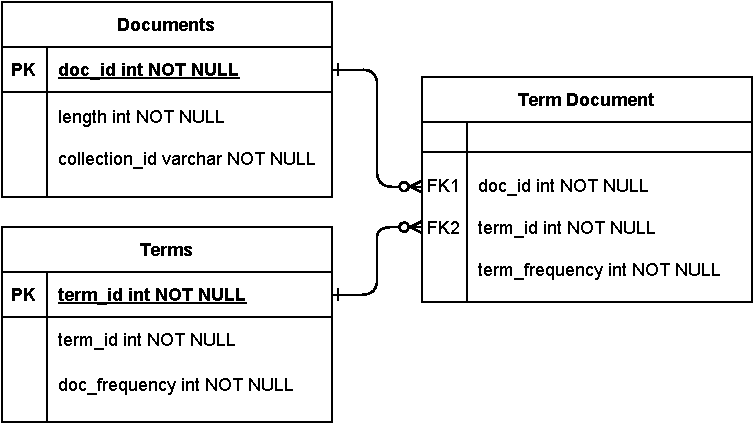
\includegraphics[width=\linewidth]{./imgs/olddog-schema-2.pdf}
	\caption{Database schema by M\"{u}hleisen et al.~for full text search in relational databases}
	\label{olddog_schema}
\end{figure}
(One for all term information, one for all document information, and one that contains the information on how terms relate to documents; the information that is found in a posting list of an inverted index). Using these three tables they show that BM25 can be easily expressed as a SQL query, with latencies that are on par with custom-build IR engines. In GeeseDB we use the exact same relational schema for full text search.
Instead of seeing the document data and term data as tables that relate to each other through a many-to-many join table, it is also possible to consider this schema as a bipartite graph. In this graph both documents and terms are considered as nodes, connected to each other through edges. Basically, if a term occurs in a document there exists an edge between that term and document. GeeseDB uses the data model of property graphs; labeled multigraphs where both edges and nodes can have property-value pairs. The database schema as described in Figure~\ref{olddog_schema} would then translate to the property graph schema shown in Figure~\ref{olddog-graph-schema}.
\begin{figure}[!h]
	\centering
	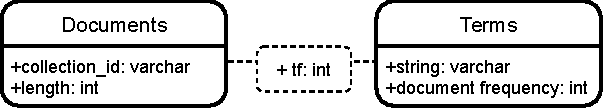
\includegraphics[width=\linewidth]{./imgs/olddog-graph-schema.pdf}
	\caption{Graph schema representing bipartite document-term graph}
	\label{olddog-graph-schema}
\end{figure}
A small example of a graph represented by this schema is shown in Figure~\ref{example-olddog-graph}, document nodes contain document specific information (i.e. document length and the collection identifier), term nodes contain information relevant to the term (i.e. the term string and the term's document frequency), and the the edges between document and terms nodes contain term frequency information (i.e. how often is the term mentioned in the document represented the respective nodes it connects).
\begin{figure}[!h]
	\centering
	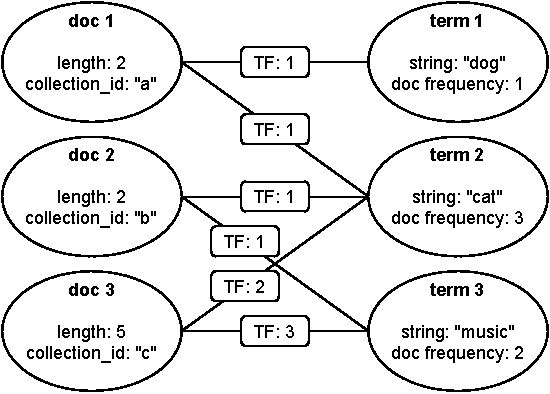
\includegraphics[width=\linewidth]{./imgs/example_olddog_graph.pdf}
	\caption{Example term-document graph that maps to relational database schema}
	\label{example-olddog-graph}
\end{figure}
If one wants to for example also store position data, this graph can easily be changed to a graph where the edges store the position of a term. If a term would appear multiple times in a document, the property graph model would allow for multiple edges to exist between two nodes. The graph schema that we described by Figure~\ref{olddog-graph-schema} maps one-to-one to the relational database schema described by Figure~\ref{olddog_schema}, so nodes are represented by normal relational tables that represent specific data units (terms, documents), while edges are represented by many-to-many join tables. So even though we think of the data as graphs, in the backend they are represented as relational tables. When using GeeseDB for search we at least expect the document-term graph to be present, of course new node types can be introduced in order to explore new search strategies. 

\subsection{Backend}
GeeseDB is built on top of DuckDB~\cite{duckdb}, an in-process SQL OLAP (analytics optimized) database management system. DuckDB is designed to support analytical query workloads, meaning that it specifically aims to process complex long-running queries where a significant portion of the data is accessed, conditions matching the case of IR research. DuckDB has a client Python API which can be installed using \texttt{pip}, afterwards it can be used directly. DuckDB has a separated API built around both NumPy and Pandas, providing NumPy/Pandas views over the same underlying data representation, without incurring data transfer (usually referred to as ``zero-copy'' reading). Pandas DataFrames can be registered as virtual tables, allowing to directly query the data present in Pandas DataFrames. GeeseDB inherits all these functionalities from DuckDB.

As DuckDB is a SQL database management system, we can execute analytical SQL queries on the tables that contain our data, including the BM25 rankings described by M\"uhleisen et al.~\cite{OldDog}. By default, the BM25 implementation provided with GeeseDB implements the disjunctive variant of BM25, instead of the conjunctive variant they used. Although the conjunctive variant of BM25 can be calculated more quickly, we chose to use the disjunctive variant as it is more commonly used by IR researchers and the differences between effectiveness scores are noticeable on smaller collections. For now we only support the original formulation of BM25 by Robertson et al.~\cite{bm25-robertson}, however support of or adding other versions of BM25~\cite{Kamphuis2020BM25} is trivial.

\section{Graph Query Language}
What distinguishes GeeseDB from alternatives, database-backed (OldDog)~\cite{olddog-docker} or native systems (Anserini~\cite{anserini}, Terrier~\cite{terrier}) is the graph query language, based on Cypher~\cite{cypher}. 
For now, GeeseDB implements Cypher's basic graph pattern matching queries for retrieving data. An example of a graph query supported by GeeseDB is presented in Figure~\ref{fig:graph_query}.
\begin{figure}
	\begin{minted}[linenos]{cypher}
MATCH (d:docs)-[]-(:authors)-[]-(d2:docs)
WHERE d.collection_id = "96ab542e"
RETURN DISTINCT d2.collection_id
	\end{minted}
	\caption{An example cypher query that finds all documents that were written by the same author that wrote the document with the \texttt{collecion\_id} ``96ab542e''}
	\label{fig:graph_query}
\end{figure}
This query finds all documents written by the same authors as those who wrote document ``96ab542e''. For comparison, Figure~\ref{fig:corresponding_sql} illustrates the same query represented in SQL; much more complex than the Cypher version, due to the join conditions that have to be made explicit. In order to connect the ``docs'' table with the ``authors'' table 2 joins are needed, reconnecting the ``docs'' table again introduces two more joins.

\begin{figure}
	\begin{minted}[linenos]{sql}
SELECT DISTINCT d2.collection_id
FROM docs AS d2
JOIN doc_author AS da2 ON (d2.collection_id = da2.doc)
JOIN authors AS a2 ON (da2.author = a2.author)
JOIN doc_author AS da3 ON (a2.author = da3.author)
JOIN docs AS d ON (d.collection_id = da3.doc)
WHERE d.collection_id = '96ab542e'
	\end{minted}
	\caption{SQL query that corresponds to the graph query described in Figure~\ref{fig:graph_query}.}
	\label{fig:corresponding_sql}
\end{figure}

At the moment of writing, GeeseDB supports the following Cypher keywords: \texttt{MATCH}, \texttt{RETURN}, \texttt{WHERE}, \texttt{AND}, \texttt{DISTINCT}, \texttt{ORDER BY}, \texttt{SKIP}, and \texttt{LIMIT}. Instead of using \texttt{WHERE} to filter data, it is also possible to use graph matching, as shown in Figure~\ref{fig:graph_query2}; the query returns the length of document ``96ab542e''. 
\begin{figure}
	\begin{minted}[linenos]{cypher}
MATCH (d:docs {d.collection_id: "96ab542e"})
RETURN d.len
	\end{minted}
	\caption{Graph query where the length of document with \texttt{collection\_id} is returned.}
	\label{fig:graph_query2}
\end{figure}
We plan to support the other keywords of Cypher in the future, as well as directed edges. Everything that is not yet directly supported yet by our implementation can of course still be expressed in SQL, which is fully supported. \footnote{GeeseDB supports the graph queries by translating them to their corresponding SQL queries, both nodes and edges are after all just tables in the backend.} In order to know how to join nodes to each other if no edge information has been provided, GeeseDB stores information on the schema. This way GeeseDB knows how nodes relate to each other through which edges. GeeseDB has a module for updating the graph schema, allowing researchers to easily set up the graph they want represented in the database.

\section{Usage}
GeeseDB comes as an easy-to-install Python package that can be installed using pip, the standard package installer for Python:

\begin{verbatim}
	$ pip install geesedb==0.0.1
\end{verbatim}
After installing GeeseDB we can immediately start using it. All examples we show in this paper were run on version v0.0.1 of GeeseDB. However, as GeeseDB is actively being developed we advise readers to use the latest version of GeeseDB, which can be installed when not specifying a package version. It is also possible to install the latest commit by installing the latest version directly from GitHub.
As an example, we will show how to use GeeseDB for the background linking task of the TREC News Track~\cite{soboroff2018trec}. The goal of this task is: \textit{Given a news story, find other news articles that can provide important context or background information.} These articles can then be recommended to the reader to help them understand the context in which these news articles take place. The collection used for this task is the Washington Post V3 collection\footnote{\url{https://trec.nist.gov/data/wapost/}} released for the 2020 edition of TREC. It contains $671.945$ news articles published by the Washington Post published between 2012 and 2020, and 50 topics with relevance assessments (topics correspond to collection identifiers of documents for which relevant data has to be found). The articles in this collection contain useful metadata; in particular, we will use authorship information. We extracted $25.703$ unique article authors, where it is possible that multiple authors co-wrote a news article. We also annotate documents with entity information which was obtained by using the Radboud Entity Linker~\cite{van2020rel}. In total $31.622.419$ references to $541.729$ unique entities were found, the links also contain mention and location information, as well as the \texttt{ner\_tag} found by the linker's entity recognition module (The \texttt{ner\_tag} is part of a link, as the entity linker can assign different tags to the same entity).\footnote{The annotated data will be made publicly available.} Figure~\ref{fig:geesedb-graph} illustrates the data schema that we use for the background linking task. 

\begin{figure}
	\centering
	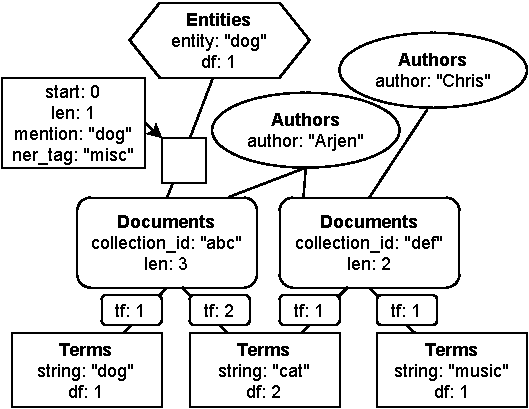
\includegraphics[width=\linewidth]{./imgs/example_full_graph.pdf}
	\caption{Example property graph for the TREC News Track's background linking task. The node types are authors, entities, terms and documents. Edges connect document nodes to other types of nodes. Both edges and nodes can have properties (following the property graph model). Multiple edges may exist between one entity node and one document node, as one entity can be linked multiple times to one document.}
	\label{fig:geesedb-graph}
\end{figure}

\subsection{Indexing and Search}
In order to start, a database containing at least the document and term information needs to be created. Figure \ref{fig:load_text_data} shows how the data can be easily loaded using CSV files.
\begin{figure}
	\begin{minted}[linenos]{python}
from geesedb.index import FullTextFromCSV

index = FullTextFromCSV(
	database='/path/to/database',
	docs_file='/path/to/docs.csv',
	term_dict_file='/path/to/term_dict.csv',
	term_doc_file='/path/to/term_doc.csv'
)
index.load_data()
	\end{minted}
	\caption{Load text data from the WashingtonPost collection formatted as csv files in the format as described by M\"uhleisen et al.~\cite{OldDog}}
	\label{fig:load_text_data}
\end{figure}

Instead of loading the data from CSV files it is also possible to load the text data directly using the CIFF format for data exchange~\cite{ciff}. GeeseDB also has functionalities to create the CSV files used here from the CIFF format. Authorship information and entity links can be loaded similarly. After loading the data we can quickly create a BM25 ranking for ad hoc search in the Washington Post collection as shown in Figure~\ref{fig:code_bm25_ranking}.

\begin{figure}
	\begin{minted}[linenos]{python}
from geesedb.search import Searcher

searcher = Searcher(
	database='/path/to/database', 
	n=10
)
hits = searcher.search_topic('obama and trump')
	\end{minted}
	\caption{Example on how to create a BM25 ranking for the query ``obama and trump'' that returns the top 10 documents.}
	\label{fig:code_bm25_ranking}
\end{figure}

For the background linking task however, we do not have regular topics; we only have the collection identifiers of the documents we need to find relevant background info for. In order to search for relevant background reading, queries that represent our information need to be constructed. A common approach is to use the top-$k$ TF-IDF terms of the source article. These can easily be found using the Cypher statement shown in Figure~\ref{fig:tfidf-cypher}. Instead of using Cypher it would also be possible to use SQL, as shown in Figure~\ref{fig:tfidf}; however this example shows again the Cypher query is more elegant. 

\begin{figure}
	\begin{minted}[linenos, escapeinside=||]{cypher}
MATCH (d:docs {collection_id: |?|})-[]-(t:term_dict)
RETURN string
ORDER BY tf*log(671945|/|df)
DESC
LIMIT 5
	\end{minted}
	\caption{Prepared Cypher statement that finds the top-$5$ TF-IDF terms in a document.}
	\label{fig:tfidf-cypher}
\end{figure}
\begin{figure}
	\begin{minted}[linenos]{sql}
SELECT term_dict.string
FROM term_dict
JOIN term_doc ON 
	(term_dict.term_id = term_doc.term_id)
JOIN docs ON 
	(docs.doc_id = term_doc.doc_id)
WHERE docs.collection_id = ?
ORDER BY term_doc.tf * log(671945/term_dict.df
DESC
LIMIT 5;
	\end{minted}
	\caption{Prepared SQL statement that finds the top-$5$ TF-IDF terms in a document.}
	\label{fig:tfidf}
\end{figure}
Processing Cypher queries depends on the schema information that needs to be loaded as well. We have a supporting class for this, and the schema data used in this paper will be available via GitHub. Using the terms found with Cypher, we can construct queries that we can pass to the searcher, and create a BM25 ranking. The code that generates the rankings for all topics is presented in Figure~\ref{fig:code_bm25_background_linking}. As you can see, with only a limited number of lines of Python code it is quite easy to create rankings. From this point it is quite trivial to write the content of \texttt{hits} to a runfile, and evaluate using \texttt{trec\_eval}. 

\begin{figure}
	\begin{minted}[linenos, breaklines]{python}
from geesedb.search import Searcher
from geesedb.connection import get_connection
from geesedb.resources import get_topics_backgroundlinking
from geesedb.interpreter import Translator

db_path = '/path/to/database'
	searcher = Searcher(
	database=db_path, 
	n=1000
)

translator = Translator(db_path)
c_query = """cypher TFIDF query"""

query = translator.translate(c_query)
cursor = get_connection(db_path).cursor
topics = get_topics_backgroundlinking(
	'/path/to/topics'
)
for topic_no, collection_id in topics:
	cursor.execute(query, [collection_id])
	topic = ' '.join(cursor.fetchall()[0])
	hits = searcher.search_topic(topic)
	
	\end{minted}
	\caption{Create a BM25 ranking for all background linking topics using the top-$5$ TFIDF terms. Note that in this case a processed topic file was used that only contains the topic identifier and the topic article id. The topic file in this format is provided on our GitHub.}
	\label{fig:code_bm25_background_linking}
\end{figure}

\noindent Instead of ``just'' ranking with BM25, using e.g.\ the metadata in order to adapt the ranking is straightforward. In the case of background linking, it makes sense to consider authorship information when recommending articles that might be suitable as background reading. As journalists are often specialized in certain news topics (e.g.\ politics, foreign affairs, tech), the stories they write often share context. Also, when journalists collaborate on stories they write together on topics they specialize in as well. As authorship information is available to us, we can decide to use the information whether an article is written by the authors of the topic article, or by someone they have collaborated with in the past. Finding the articles that are written by this group of people can easily be done using a graph query, the query that finds these articles is shown in Figure~\ref{fig:author-cypher}.

\begin{figure}
	\begin{minted}[linenos, breaklines, breakafter=-, escapeinside=||]{cypher}
MATCH (d:docs)-[]-(:authors)-[]-(:docs)-[]-(:authors)-[]-(d2:docs {collection_id: |?|}) 
RETURN DISTINCT d.collection_id
	\end{minted}
	\caption{Cypher query to find documents written by co-authors of the authors of the topic article.}
	\label{fig:author-cypher}
\end{figure}

\noindent Depending on the number of documents found by this query, different rescoring strategies can be decided upon. If the set of documents written by the authors or their co-authors is large, perhaps it is possible to only consider these documents, but if the set is small, a score boost might be more appropriate. Figure~\ref{fig:authors-code} shows an example on how to only consider documents found with the query in Figure~\ref{fig:author-cypher}, in this particular case we ensure that at least 2000 documents are found before filtering.

\begin{figure}
	\begin{minted}[linenos, breaklines]{python}
# import and first lines the same as previous example

author_c_query = """cypher authorship query"""
author_query = t.translate(author_c_query)

cursor = get_connection(db_path).cursor
topics = get_topics_backgroundlinking(
	'/path/to/topics'
)
for topic_no, collection_id in topics:
cursor.execute(query, [collection_id])
topic = ' '.join(cursor.fetchall()[0])
hits = searcher.search_topic(topic)

cursor.execute(author_query, [collection_id])
docs_authors = {
	e[0] for e in cursor.fetchall()
}
if len(docs_authors) > 2000:
	hits = hits[hits.collection_id.isin(docs_authors)]
	\end{minted}
	\caption{Find documents written by all authors that collaborated with the authors of the topic article, if there are more than 2000 documents found only consider these documents as background reading candidates.}
	\label{fig:authors-code}
\end{figure}

To give another example; the graph query language is also useful when considering entities. When journalists write news articles, the articles relate to events concerning e.g.\ people, organisations, or countries. In other words, the basis of news articles lay the entities as they are often the subject of news. So, instead of using the most informative terms in a news article, it could be useful to consider the entities identified in the article instead. Important entities tend to be mentioned in the beginning of a news article~\cite{entities-loc}; Figure~\ref{fig:entity-cypher} shows the Cypher query to retrieve the text mentions of the first five mentioned entities.

\begin{figure}
	\begin{minted}[linenos, breaklines, breakafter=-, escapeinside=||]{cypher}
MATCH (d:docs {collection_id: |?|})-[]-(e:entities)
RETURN mention
ORDER BY |start|
LIMIT 5
	\end{minted}
	\caption{Retrieve the first five entities mentioned in the topic article; and return the terms used to mention the entity.}
	\label{fig:entity-cypher}
\end{figure}
\noindent Before it is possible to search using the text describing the first five entity mentions, the text needs to be processed. The term data loaded in GeeseDB was already processed, as it was data loaded from CSV files built from a CIFF file created from an Anserini~\cite{anserini} (Lucene) index. Anserini has an easy to use Python extension, Pyserini~\cite{pyserini}, that can be used to tokenize the text in the same way as the documents were tokenized. Figure~\ref{fig:entities-code} shows the Python code where we extract the mentions, process them such that they become a usable query for GeeseDB, and then BM25 ranking is created with this query.

\begin{figure}
	\begin{minted}[linenos, breaklines]{python}
from geesedb.search import Searcher
from geesedb.connection import get_connection
from geesedb.resources import get_topics_backgroundlinking
from geesedb.interpreter import Translator
from pyserini.analysis import Analyzer, get_lucene_analyzer

db_path = '/path/to/database'
	searcher = Searcher(
	database=db_path,
	n=1000
)

analyzer = Analyzer(get_lucene_analyzer())

translator = Translator(db_path)
c_query = """cypher entity query"""
query = translator.translate(c_query)

cursor = get_connection(db_path).cursor
topics = get_topics_backgroundlinking(
	'/path/to/topics'
)

for topic_no, collection_id in topics:
cursor.execute(query, [collection_id])
topic = ' '.join([e[0] for e in cursor.fetchall()])
topic = ' '.join(analyzer.analyze(topic))
hits = searcher.search_topic(topic)
	\end{minted}
	\caption{Create a BM25 ranking for all background linking topics using the mention text of the first five linked entities in the source article.}
	\label{fig:entities-code}
\end{figure}

\section{Conclusion}
